\chapter{Цель и задачи}
\label{ch:intro}

\textbf{Цель}: Исследовать свойства конечной дискретной,
однородной цепи Маркова. Оценить параметры распределения числа
коммутаций пакетов в сети.

\section*{Задание к лабораторной работе}

\begin{figure}[H]
    \centering
    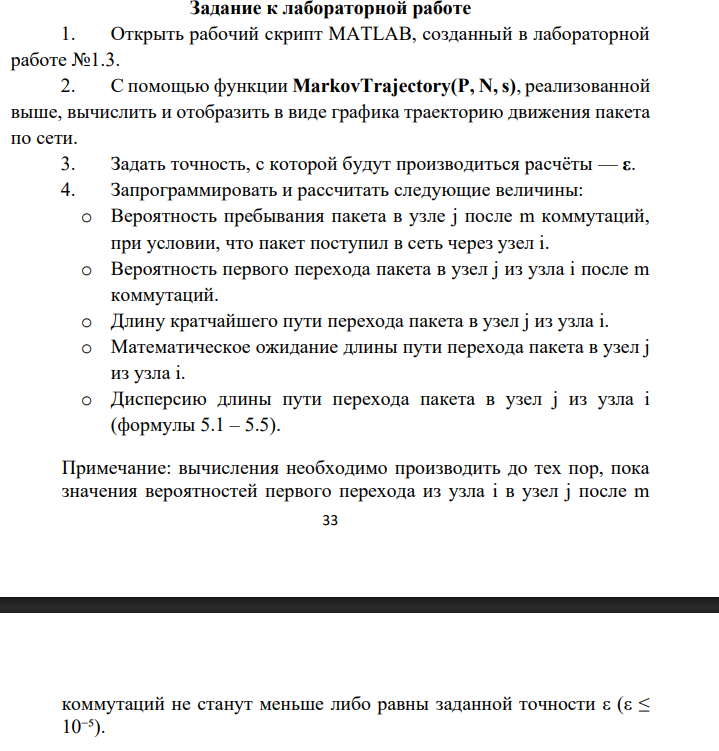
\includegraphics[width=1.0\textwidth]{task1.png}
    \caption{Задание для лабораторной работы}
\end{figure}

\begin{figure}[H]
    \centering
    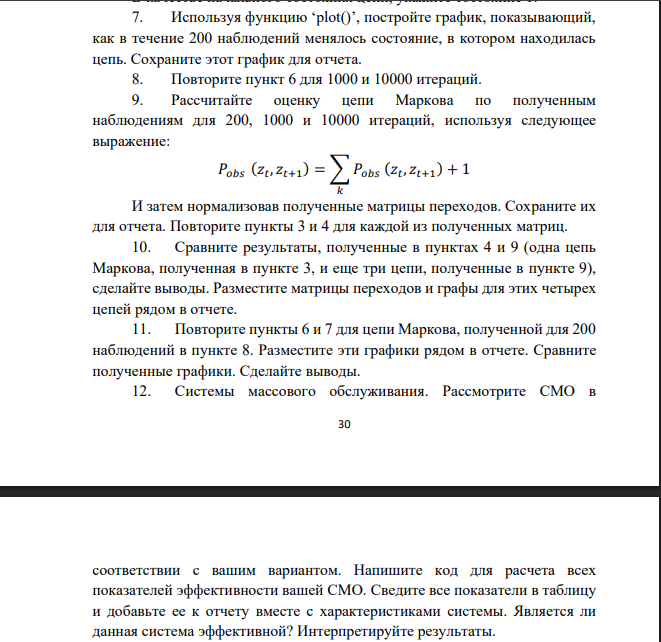
\includegraphics[width=1.0\textwidth]{task2.png}
    \caption{Задание для лабораторной работы}
\end{figure}

\endinput